With the statistical and analytic machinery in place, the results are 
rather straight-forward. However, the results are also rather striking. 
First, as discussed in Section \ref{sec:Methods}, we computed the mixed model
given by \texttt{count ~ phase + facet + (1|date)} for 266 different date
partitions determining which date was assigned to which phase. The first
partition date ranged between September 26 and October 9, 2016. The
second partition date was between October 27 and November 14, 2016.
The phase was 1 if the date was before the first partition date, 2 if the 
date was on or after the first partition date and before the 
second partition date, or 3 if the observation date was on or after the second 
partition date.


\begin{figure}
  \centering
  % \vspace*{-.55in}
  \hspace*{-.25in}
  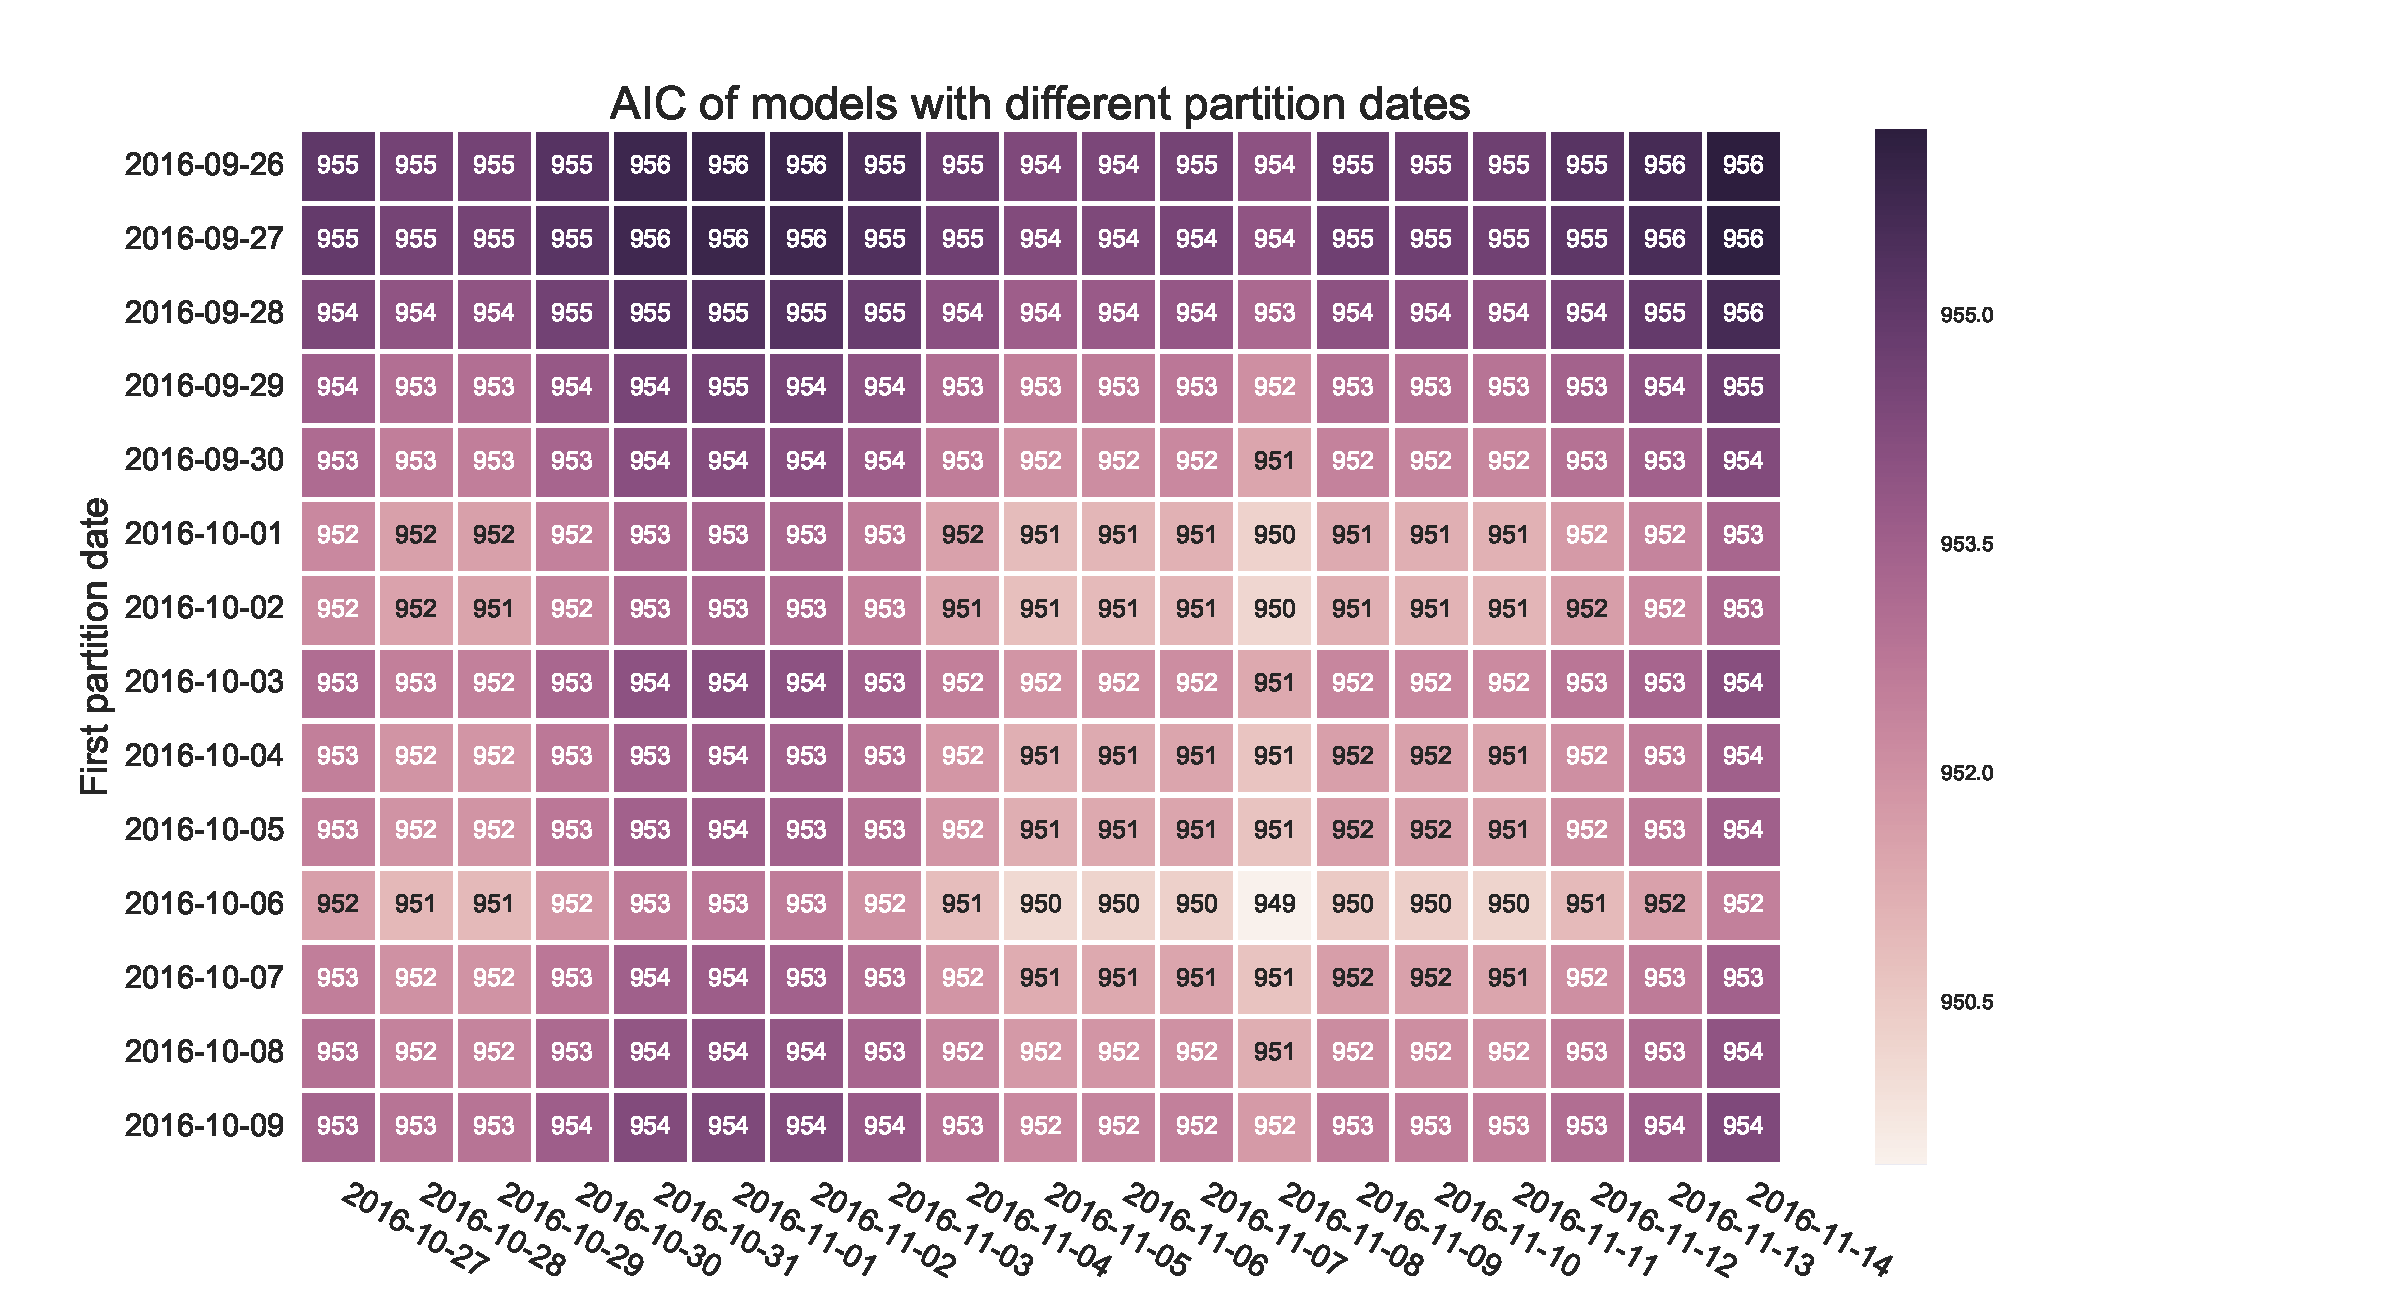
\includegraphics[width=1.25\textwidth]{figures/AIC_dates-FIG2.pdf}

\caption{
  Akaike information criterion (AIC) for models of \texttt{count ~ phase + facet + (1|date)}
  for 266 different phase assignments. The phase was 1 if the date was before
  the first partition date, 2 if the date was on or after
  the first partition date and before the second partition date, or
  3 if the observation date was on or after the second partition date.
}
\label{fig:AICs}
\end{figure}


\begin{figure}
  \centering
  % \vspace*{-.55in}
  \hspace*{-.25in}
  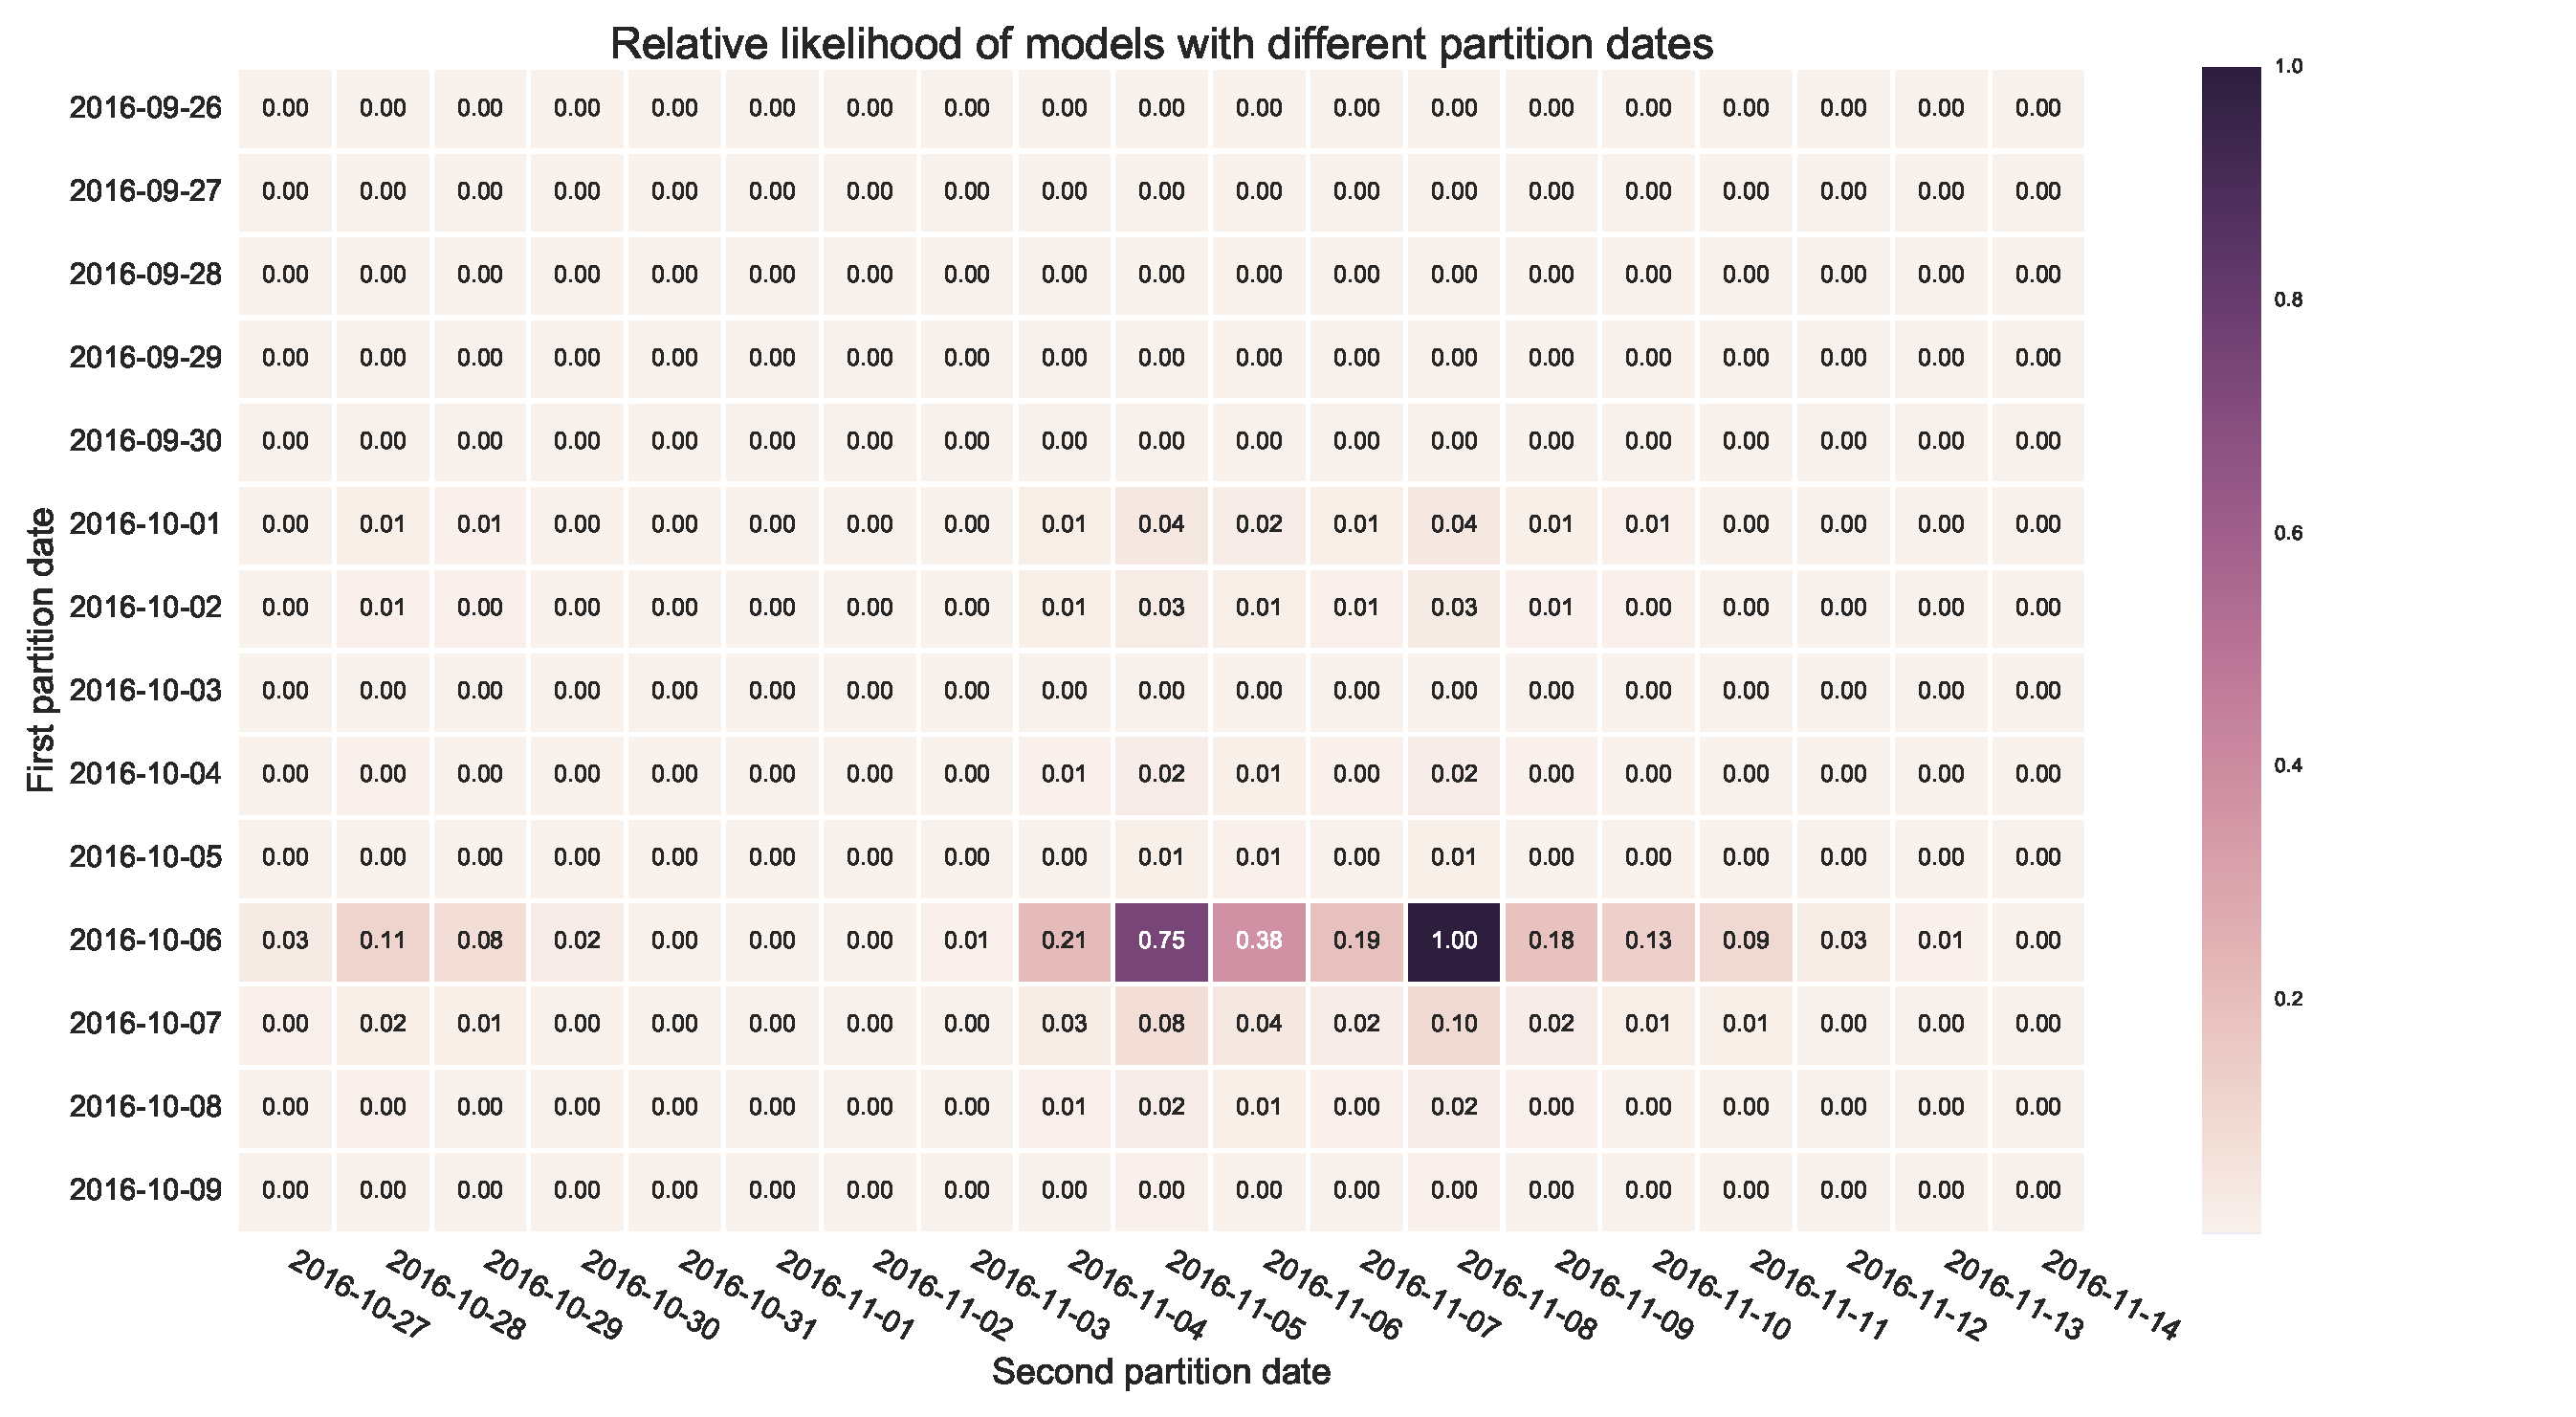
\includegraphics[width=1.25\textwidth]{figures/rel_likelihood_dates-FIG2.pdf}

\caption{
  Relative likelihood of models with identical formula, but different dates
  used to partition the data into three ``phases''. The phase 
  was 1 if the date was before
  the first partition date, 2 if the date was on or after
  the first partition date and before the second partition date, or
  3 if the observation date was on or after the second partition date.
}
\label{fig:relative-likelihoods}
\end{figure}

Recall that a model relatively higher AIC means more information was lost by
that model. So, a lower relative AIC is better. However, miniscule differences
in AIC cannot be considered conclusive. To select the model that best fits the
data, which in turn selects the dates that best correspond to the locations
of the phase transitions, we first compute the AIC of all candidate models, 
The results of this calculation for all candidate models that include phase
are shown in Figure \ref{fig:AICs}. To determine the probability that 
another model will not minimize information loss better,
the model with the minimum AIC is compared to all $N-1$ other models using
the relative likelihood, $\mathcal{L}_i$, where $i = 1, \ldots, N; i \neq i_{min}$,
where $i_{min}$ is the model index with minimum AIC. $\mathcal{L}_i$ was defined
in Equation \ref{eq:relative-likelihood}. 

The pair of partition dates with the smallest AIC was October 10 and
November 8, with an AIC of 1179. We then calculated $\mathcal{L}_i$ for all 
$N-1$ other models, 
with the results shown in Figure \ref{fig:relative-likelihoods}. At first,
we might be discouraged by the results. The first partition date,
October 10, seems to easily be the best candidate for our first partition
since there are no significantly likely alternatives
going up or down its axis in the figure. However the second partition date
with minimum AIC, November 8, is relatively less likely to be the very best one 
in terms of information loss. That is, there are alternatives that are nearly 
as likely to minimize information loss, with the first significant candidates
coming as early as October 28$^{th}$ and 29$^{th}$ with a relative likelihood of 
.11 and .08, respectively. In the four days before November 8$^{th}$, the likelihoods
are .21, .75, .38, and .19, and the three days after have relative likelihoods
of equal or better performance of .18, .13, and .09, all significant. 

There is an alternative explanation that does not imply that our method for
identifying the location of a phase transition is not working. What if,
instead, our procedure is identifying an area of mixed phase, or a transient
phase to use more of a dynamical systems term. The transience, then, begins
lightly in late October, and begins in force November 4$^{th}$, tapering off
with the phase transition complete on November 11$^{th}$. 
